\documentclass[aspectratio=169]{beamer}

\usetheme{Madrid}
\usecolortheme{seahorse}
\setbeamertemplate{navigation symbols}{}
\setbeamertemplate{footline}[frame number]

\usepackage{amsmath}
\usepackage{tikz}
\usetikzlibrary{arrows.meta,positioning,shapes.geometric}

\title[Robust Crew Pairing]{Incremental Data-Driven Robust Crew Pairing Optimization}
\subtitle{Under Evolving Uncertainty}
\author{Xinyu HUANG}
\institute{The Hong Kong Polytechnic University}
\date{}

\begin{document}

% Parole:
% Good morning everyone. My name is Xinyu HUANG. Today I am going to introduce
% my project, called Incremental Data-Driven Robust Crew Pairing Optimization
% Under Evolving Uncertainty. The project is about airline crew pairing, which
% means deciding which crews should cover which flights. This is important
% because every flight needs qualified crew members, and the schedule must
% respect many rules, such as working time, rest time, and connection time.
% In this presentation, I will first explain the motivation, then the data-driven
% uncertainty model, then the two-stage robust optimization framework, and
% finally the incremental re-optimization idea.
\begin{frame}
  \titlepage
  \vspace{-0.35cm}
  \begin{center}
    \small Motivation $\rightarrow$ Uncertainty model $\rightarrow$ Robust optimization $\rightarrow$ Re-optimization
  \end{center}
\end{frame}

% Parole:
% The motivation comes from real airline operations. Crew pairing is already a
% large scheduling problem, because there can be many possible ways to connect
% flights into crew duties. But the problem becomes harder when delays happen.
% A flight delay may make the crew miss the next connection, and then the airline
% has to wait, swap crews, or even cancel. So the goal is not only to find a
% cheap schedule, but also to find a schedule that can remain feasible and
% recoverable when disruptions happen.
\begin{frame}{Why Crew Pairing Is Difficult}
  \begin{columns}[T,onlytextwidth]
    \column{0.48\textwidth}
      \textbf{Planning requirement}
      \begin{itemize}
        \item Every flight must be covered.
        \item Crew duties must satisfy rules.
        \item Pairing cost should be controlled.
      \end{itemize}

    \column{0.48\textwidth}
      \textbf{Operational uncertainty}
      \begin{itemize}
        \item Delays break flight connections.
        \item Recovery creates extra cost.
        \item Rare disruptions are important.
      \end{itemize}
  \end{columns}

  \vspace{0.45cm}
  \begin{block}{Project goal}
    Build a crew pairing plan that is low-cost, robust to delays, and easy to update when new data arrive.
  \end{block}
\end{frame}

% Parole:
% A central part of this project is how to describe uncertainty. A simple
% probability distribution may not be reliable, because historical data often
% contains many normal days and only a few serious disruption days. If we fit a
% normal distribution, we may underestimate the rare but operationally important
% delays. Therefore, this project uses a data-driven uncertainty set. For each
% flight, the delay bound is estimated by an empirical quantile from historical
% data. The model focuses on one-sided uncertainty, because late arrival creates
% risk, while early arrival is usually absorbed by the schedule.
\begin{frame}{Data-Driven Uncertainty Set}
  \begin{columns}[T,onlytextwidth]
    \column{0.48\textwidth}
      \textbf{Why not only fit a distribution?}
      \begin{itemize}
        \item Limited disruption data.
        \item Correlation and extreme shifts are hard to capture.
        \item Normal days can dilute serious delay events.
      \end{itemize}

    \column{0.48\textwidth}
      \textbf{Proposed idea}
      \begin{itemize}
        \item Use empirical quantiles from delay data.
        \item Model only upward delay deviations.
        \item Control conservatism through a budget.
      \end{itemize}
  \end{columns}

  \vspace{0.35cm}
  \[
    d_f = \mathrm{Quantile}_{\alpha}
    \left(x_f^1, x_f^2, \ldots, x_f^T\right),
    \qquad
    0 \leq \Delta_f \leq d_f
  \]
\end{frame}

% Parole:
% If we assume that every flight reaches its worst delay at the same time, the
% model will become too conservative. In real life, this is usually unnecessary.
% That is why the project uses a budget-of-uncertainty parameter, denoted by
% Gamma. Gamma controls how many delay components can be active at the same
% time. A small Gamma gives a cheaper but less protected schedule. A large Gamma
% gives a safer but more expensive schedule. This creates a practical trade-off
% between robustness and cost.
\begin{frame}{Balancing Robustness And Cost}
  \begin{center}
  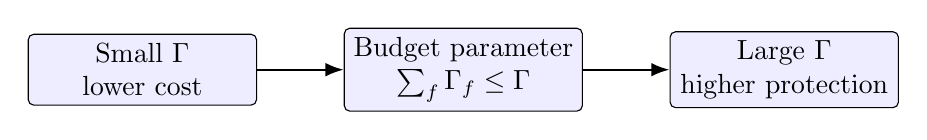
\begin{tikzpicture}[
    scale=0.95,
    box/.style={draw, rounded corners=2pt, align=center, minimum width=2.9cm,
      minimum height=0.9cm, fill=blue!7},
    arrow/.style={-Latex, thick}
  ]
    \node[box] (low) {Small $\Gamma$\\lower cost};
    \node[box, right=1.1cm of low] (mid) {Budget parameter\\$\sum_f \Gamma_f \leq \Gamma$};
    \node[box, right=1.1cm of mid] (high) {Large $\Gamma$\\higher protection};
    \draw[arrow] (low) -- (mid);
    \draw[arrow] (mid) -- (high);
  \end{tikzpicture}
  \end{center}

  \vspace{0.3cm}
  \[
    \hat{\mathcal U}(\Gamma)
    =
    \left\{\Delta: 0 \leq \Delta_f \leq d_f,\;
    \sum_f \Gamma_f \leq \Gamma,\;
    \Delta_f = \Gamma_f d_f \right\}
  \]

  \begin{itemize}
    \item Protects against serious delay scenarios.
    \item Avoids assuming all flights are delayed at once.
    \item Lets the airline tune the level of conservatism.
  \end{itemize}
\end{frame}

% Parole:
% The optimization model has two stages. In the first stage, before the actual
% disruption is known, the airline chooses the crew pairings. In the second
% stage, after a delay scenario appears, the model decides how to recover the
% schedule. The recovery actions include waiting, swapping, or cancelling. The
% objective is to minimize the planned pairing cost plus the worst-case recovery
% cost. This is a robust optimization model because it explicitly considers the
% worst scenario inside the uncertainty set.
\begin{frame}{Two-Stage Robust Optimization Model}
  \begin{columns}[T,onlytextwidth]
    \column{0.46\textwidth}
      \begin{block}{First stage: planning}
        Choose crew pairings before the actual disruption is known.
      \end{block}
      \[
        \min_x \sum_{p \in P} c_p x_p + \theta
      \]

    \column{0.50\textwidth}
      \begin{block}{Second stage: recovery}
        Under delay scenarios, choose recovery actions.
      \end{block}
      \begin{itemize}
        \item Wait and absorb delay.
        \item Swap crew or connection.
        \item Cancel when necessary.
      \end{itemize}
  \end{columns}

  \vspace{0.25cm}
  \[
    \min_x \left\{ \text{planned cost}
    + \max_{\Gamma \in \hat{\mathcal U}}
    \text{recovery cost}(x,\Gamma) \right\}
  \]
\end{frame}

% Parole:
% To solve this model, the project combines two important methods. The first is
% column generation, which is common in crew pairing because the number of
% possible pairings can be extremely large. Instead of listing all pairings, the
% algorithm adds useful pairings with negative reduced cost. The second method
% is nested column-and-constraint generation. This method adds important
% worst-case scenarios and their constraints step by step. Together, these
% methods allow the model to focus on the pairings and scenarios that matter.
\begin{frame}{Solution Algorithm}
  \begin{center}
  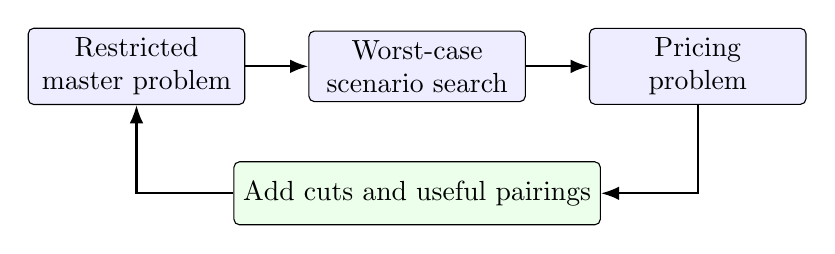
\begin{tikzpicture}[
    box/.style={draw, rounded corners=2pt, align=center, minimum width=2.75cm,
      minimum height=0.8cm, fill=blue!7},
    greenbox/.style={draw, rounded corners=2pt, align=center, minimum width=3.2cm,
      minimum height=0.8cm, fill=green!8},
    arrow/.style={-Latex, thick}
  ]
    \node[box] (rmp) {Restricted\\master problem};
    \node[box, right=0.8cm of rmp] (sp) {Worst-case\\scenario search};
    \node[box, right=0.8cm of sp] (pp) {Pricing\\problem};
    \node[greenbox, below=0.75cm of sp] (update) {Add cuts and useful pairings};

    \draw[arrow] (rmp) -- (sp);
    \draw[arrow] (sp) -- (pp);
    \draw[arrow] (pp.south) |- (update.east);
    \draw[arrow] (update.west) -| (rmp.south);
  \end{tikzpicture}
  \end{center}

  \begin{itemize}
    \item Column generation handles the large pairing space.
    \item Nested C\&CG handles mixed-integer recourse and worst-case scenarios.
    \item The algorithm stops when no useful pairing or violated scenario remains.
  \end{itemize}
\end{frame}

% Parole:
% The key contribution is incremental re-optimization. In practice, new delay
% data arrive over time, so the uncertainty set changes. If the new uncertainty
% set becomes smaller, the old robust solution is still feasible and can be
% viewed as conservative. If the uncertainty set becomes larger, we do not need
% to rebuild the whole model from zero. We can add the new robustness cuts and
% re-optimize from the previous model. This is useful for airline planning
% because the environment changes continuously.
\begin{frame}{Incremental Re-Optimization}
  \begin{columns}[T,onlytextwidth]
    \column{0.48\textwidth}
      \textbf{When uncertainty shrinks}
      \begin{itemize}
        \item New bounds are tighter.
        \item Old robust solution remains feasible.
        \item The plan is conservative but safe.
      \end{itemize}

    \column{0.48\textwidth}
      \textbf{When uncertainty expands}
      \begin{itemize}
        \item New bounds are looser.
        \item Add new robustness cuts.
        \item Re-optimize without rebuilding from zero.
      \end{itemize}
  \end{columns}

  \vspace{0.35cm}
  \begin{block}{Practical value}
    The model can adapt when operational data evolve, while reusing the previous optimization structure.
  \end{block}
\end{frame}

% Parole:
% To conclude, this project proposes a robust crew pairing framework that is
% data-driven and adaptive. It uses quantile-based delay bounds to describe
% uncertainty, a budget parameter to balance robustness and cost, and a
% two-stage robust optimization model to include recovery decisions. The
% algorithm combines nested column-and-constraint generation with column
% generation, so it can add only important scenarios and useful pairings. Most
% importantly, the incremental re-optimization mechanism allows the model to
% update efficiently when new delay data arrive. This makes the approach more
% suitable for real airline operations. Thank you for listening.
\begin{frame}{Conclusion}
  \begin{itemize}
    \item Crew pairing needs schedules that are feasible, low-cost, and robust.
    \item Quantile-based uncertainty sets use historical delay data directly.
    \item Two-stage robust optimization models planning and recovery together.
    \item Nested C\&CG and column generation solve the model iteratively.
    \item Incremental re-optimization updates the model as uncertainty evolves.
  \end{itemize}

  \vspace{0.35cm}
  \begin{block}{Final takeaway}
    A robust, data-driven, and adaptive framework for airline crew pairing under evolving delay uncertainty.
  \end{block}
\end{frame}

\end{document}
